\begin{figure}[H]
    \begin{minipage}[b]{0.3\linewidth}
        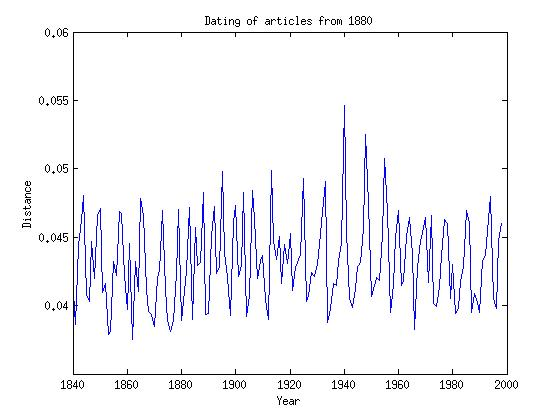
\includegraphics[scale=0.25]{Pictures/date_articles/cos/dating1880.jpg}
        \caption{Dating articles from 1880 with the cosine distance}
    \end{minipage}\hfill
    \begin{minipage}[b]{0.3\linewidth}
        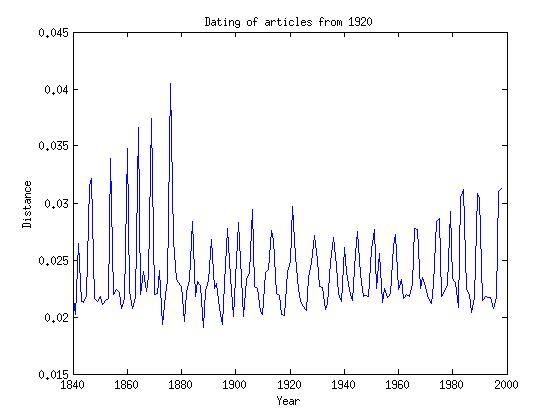
\includegraphics[scale=0.25]{Pictures/date_articles/cos/dating1920.jpg}
        \caption{Dating articles from 1920 with the cosine distance}
    \end{minipage}\hfill
    \begin{minipage}[b]{0.3\linewidth}
	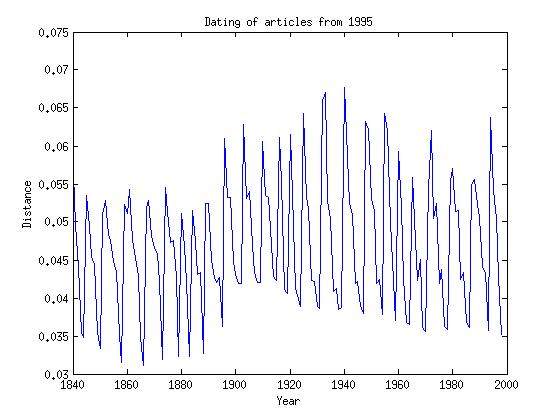
\includegraphics[scale=0.25]{Pictures/date_articles/cos/dating1995_corrected.jpg}
        \caption{Dating articles from 1995 with the cosine distance}
    \end{minipage}
    \label{date_d1}
\end{figure}
The cosine distance looks also relatively random for dating. For the example in figure \ref{date_cos}, the prediction is 1852 where the articles come from 1995.